Given $n$ cities that the traveling sellsman want to do business, matrix $M$ where $M_{ij}$ is the distance from city $i$ to city $j$. The goal is to find a tour of $n$ cities returning to the starting cities of least total cost.

Describe the problem mathematically, find a permutation $\sigma$ of $1 \cdots n$ so as to minimize \[\sum_{i=0}^{n-1} M[\sigma(i), \sigma(i+1)] + M[\sigma(n), \sigma(1)]\]

This is a NP-hard problem. 

The decision problem is NP complete:
\begin{itemize}
	\item Instance: matrix $M$ and a budge $B$
	\item Question: is there a tour of the cities with cost at most $B$.
\end{itemize}

The problem is in NP. Given a permutation of cities as certificate, we can check the cost in order and sum the cost up to see if it is lower than the given budge. It can be finished within polynomial time.

Prove NP-complete by a reduction from Hamilton cycle (HAMCYCLE).

The Hamilton cycle decision problem(HAMCYCLE):
\begin{itemize}
	\item Instance: directed graph $G$
	\item Question: is there a simple cycle containing all the vertices? (such cycle is called a Hamilton cycle)
\end{itemize}

Exercise: HAMCYCLE $\preccurlyeq_P$ TSP.

\subsection{Approximation Algorithm TSP OPT}
Don't know a good approximation for a general TSP.  But we are able to approximate Metric -TSP. Metric TSP is as follow:
\begin{itemize}
	\item Input: matrix $M$ of costs. $M$ satisfies the property of a metric:
	\begin{itemize}
		\item $M[i, i] = 0$
		\item $M[i, j] = M[j, i]$
		\item $M[i, k] \le M[i, j] + M[j, k], \forall i, j, k$.
	\end{itemize} 
\end{itemize}
 
OPT(M) is the cost of the best tour for a given matrix $M$. Design algorithm $A$. We say $A(M)$ is the cost of tour that $A$ outputs. We want $\forall M, \frac{A(M)}{OPT(M)} \le C$. Can achieve $c = 2$.

Suppose we have a best tour, when we delete one edge from the tour, what do we have? We get a Hamilton path which goes through all the cities. The path is a tree on all the vertices in the graph, i.e. a spanning tree. The cost this spanning tree (path) $\le$ cost of the tour. So cost of MST $\le$ cost of the spanning tree $\le$ cost of the optimal tour.

Approximation algorithm:
Think of $M$ as a weighted, connected,  undirected graph. Find the MST in the graph, call it $T$. Duplicate every edge in $T$. Cost of $T$ $\le$ cost of OPT. The cost of duplicated tree = 2 $\times$ cost$(T)$.

Because of the duplication, every vertex has even degree. So any connected undirected graph with all degrees even has an Eulerian tour. Eulerian tour is a tour that goes though all the edges of the graph exactly once. We can find Eulerian efficiently in order $O(m+n)$ time using DFS.

\begin{figure}[H]
	\centering
	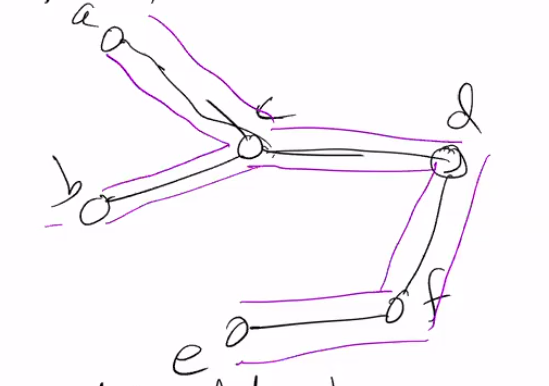
\includegraphics[width=0.5\textwidth]{fig/eulerian-tour.png}
\end{figure}

The Eulerian tour in the above graph is $(a, c, d, f, e, f, d, c, b, c, a)$. 

The cost of Eulerian tour = $2 \times$ MST $\le$ 2 OPT($M$). So it turns out the Eulerian tour is a nice tour with the cost less than 2 OPT($M$). But we cannot use Eulerian as the output since the real undirected graph does not have duplicate edges. But it is easy to generate Hamilton path from Eulerian tour by skip the duplicates. To be more specific, drop the edges in Eulerian tour as long as it has been seen before.

Therefore the Hamilton tour is $(a, c, d, f, e, \cancel{f, d, c,} ~b~\cancel{, c, a})$

\textbf{Claim}: Removing duplicate occurrences of vertices in the Eulerian tour dose not increase the cost of the tour.

\begin{proof}
	\begin{figure}[H]
		\centering
		
\includegraphics[width=0.3\textwidth]{fig/trangle.png}
	\end{figure}
If we remove $c$ from the graph and connect b to a, recall that this is a metric matrix so the triangle rules applies. $M[b, a] \le M[b, c] + M[c, a]$.

We then use induction to prove that $(e,b)$ is less than $(b, c, d, f, e)$.
\begin{figure}[H]
	\centering
	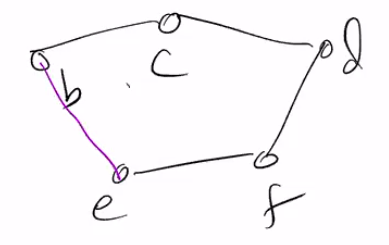
\includegraphics[width=0.3\textwidth]{fig/trangle-short-path.png}
\end{figure}

First of all, if we only skip vertex $f$ by connecting $e$ to $d$. $(e, d)$ would be better than $(e, f, d)$ by triangle rules. Then use the same idea again . $(e, c)$ would be at most expensive as $(e, d, c)$. Then finally $(e,b)$ is better than $(e, c, b)$. This applies more generally for a sequence of vertex deletion.
\end{proof}
\subsubsection{Appro Algorithm}
\begin{itemize}
	\item Find MST ($\le$ OPT)
	\item Duplicate edges ($\le$ 2 OPT)
	\item Find Eulerian tour ($\le$ 2 OPT)
	\item Convert to Hamilton tour (or TSP tour) by skipping duplicate visits to vertices. ($\le$ 2 OPT)
\end{itemize}
This is a 2-approximation algorithm.



\subsection{Improvments}
\subsubsection{Christofides}
Metric-TSP can be approximate even better than 2-approximation. The best known approximation is \textbf{1.5-approximation} for metric-TSP by Christofides Algorithm. 
\begin{itemize}
	\item Find MST ($\le$ OPT)
	\item Christofides: find the min-cost perfect matching on the odd degree vertices. Add it to the MST. Now all the vertices become even degree. ($\le$ 1.5 OPT)
	\item Find Eulerian tour ($\le$ 2 OPT)
	\item Convert to Hamilton tour (or TSP tour) by skipping duplicate visits to vertices. ($\le$ 2 OPT)
\end{itemize}

\begin{figure}[H]
	\centering
	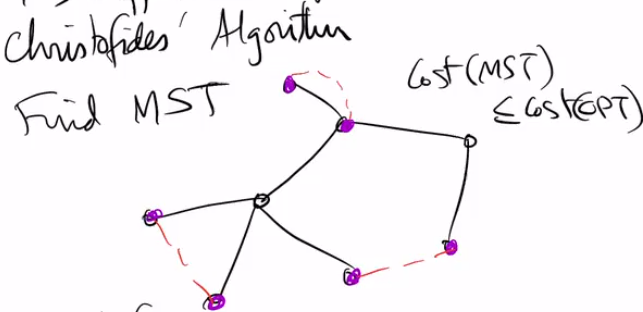
\includegraphics[width=0.5\textwidth]{fig/christofides.png}
\end{figure}
\subsubsection{Approximation Scheme}
Approximation Scheme: given any $\epsilon$ as input, there is an algorithm that always find a solution that is at most $(1 + \epsilon)$ time OPT. Running time of the algorithm grows as a polynomial function of $\frac{1}{\epsilon}$.




















